\chapter{Development of Analytical Approach}

\section{Purpose}
Review a selection of my contributions to the literature that have informed the approach used in this project throughout my tenure as a member of the lab
\begin{enumerate}
 \item Comparative genomics allows the discovery of cis-regulatory elements in mosquitoes
  \begin{itemize}
   \item Use of comparative genomics to discover putative CREs from orthologous promoter regions in mosquitoes that were able to be corelated with bloodmeal associated transcription control
  \end{itemize}
 \item RNA-seq analyses of blood-induced changes in gene expression in the mosquito vector species, Aedes aegypti
  \begin{itemize}
   \item relevance
  \end{itemize}

 \item Strain Variation in the Transcriptome of the Dengue Fever Vector, Aedes aegypti
   \begin{itemize}
   \item relevance
  \end{itemize}
 \item Comparative Transcriptome Analyses of Deltamethrin-Resistant and-Susceptible Anopheles gambiae Mosquitoes from Kenya by RNA-Seq
   \begin{itemize}
   \item relevance
  \end{itemize}
 \item Complex Modulation of the Aedes aegypti Transcriptome in Response to Dengue Virus Infection
   \begin{itemize}
   \item relevance
  \end{itemize}
\end{enumerate}

\section{Comparative genomics allows the discovery of cis-regulatory elements in mosquitoes}

See Figure \ref{fig:sieglaff2009_full}
Figure \ref{fig:mosqPhyloTree}


\begin{figure}[h]

\hfil
\includegraphics[scale=.95]{figures/figs/sieglaff2009_full.pdf}
\hfil
\caption[Associations of mosquito motifs with gene expression profiles in \Ag]{\bsf{Associations of mosquito motifs with gene expression profiles in \Ag:} \\ \sf
Motif enrichment within (A) 5′-end flanking regions of genes in clusters responsive to blood meal ingestion, and in (B) 5′-end flanking regions of genes in clusters enriched in selected tissues. The significance of motif enrichment is indicated by pseudocolor of -log10 (P-value) determined through hypergeometric statistics, and the median expression profile of each gene cluster is shown below each respective column. Red and green colors represent higher and lower relative mRNA accumulation, respectively. Asterisks (*) indicate a match to a previously described mosquito TFBS. Heatmaps were created with Matrix2png (\CITEME:local-58). FB, fat body; hPBM, hours post blood meal; MG, midgut; OV, ovaries; TC, time course clusters.

Adapted from \cite{Sieglaff2009}}
\label{fig:sieglaff2009_full}
\end{figure}

\begin{figure}[hp]
\centering

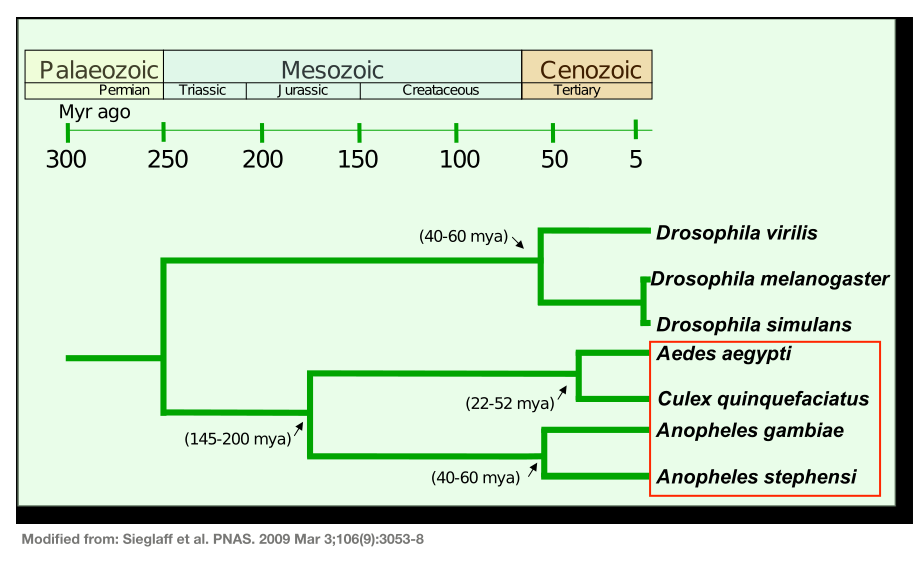
\includegraphics[width=.7\textwidth]{figures/figs/mosqPhyloTree.pdf}

\caption[Phylogenetic relationships between four vector mosquitoes]{\bsf{Phylogenetic relationships between four vector mosquitoes compared with representative \textit{Drosophila} species.} 

Adapted from \cite{Sieglaff2009}}
\label{fig:mosqPhyloTree}
\end{figure}

%%% Local Variables: ***
%%% mode: latex ***
%%% TeX-master: "thesis.tex" ***
%%% End: ***
